\chapter{Supplement -- Thesis Structure as a Taskflow}
\label{App_C:ThesisWorkflow}
\chaptertoc

\section{Structuring the thesis as a task flow}
\label{App_C_sec:intro_taskflow}

This Appendix shows the structure of this thesis outlined as a task flow, where the thesis's main points, keywords, or key paragraphs are described as a task. There are five figures shown here, including:
\begin{itemize}
	\item Figure \ref{fig:thesistaskflow_chapter1}: the taskflow of Chapter 1 - Introduction.
	\item Figure \ref{fig:thesistaskflow_chapter2}: the taskflow of Chapter 2 - From work stealing to reactive load balancing, associated with related works.
	\item Figure \ref{fig:thesistaskflow_chapter3}: the taskflow of Chapter 3 - Performance modeling and analysis.
	\item Figure \ref{fig:thesistaskflow_chapter4}: the taskflow of Chapter 4 - A proactive approach for dynamic load balancing.
	\item Figure \ref{fig:thesistaskflow_chapter567}: the taskflows of Chapters 5, 6, 7 - Corresponding to proof of concepts, evaluation, and conclusions in this thesis.
\end{itemize}

\begin{figure}[t]
  \centering
  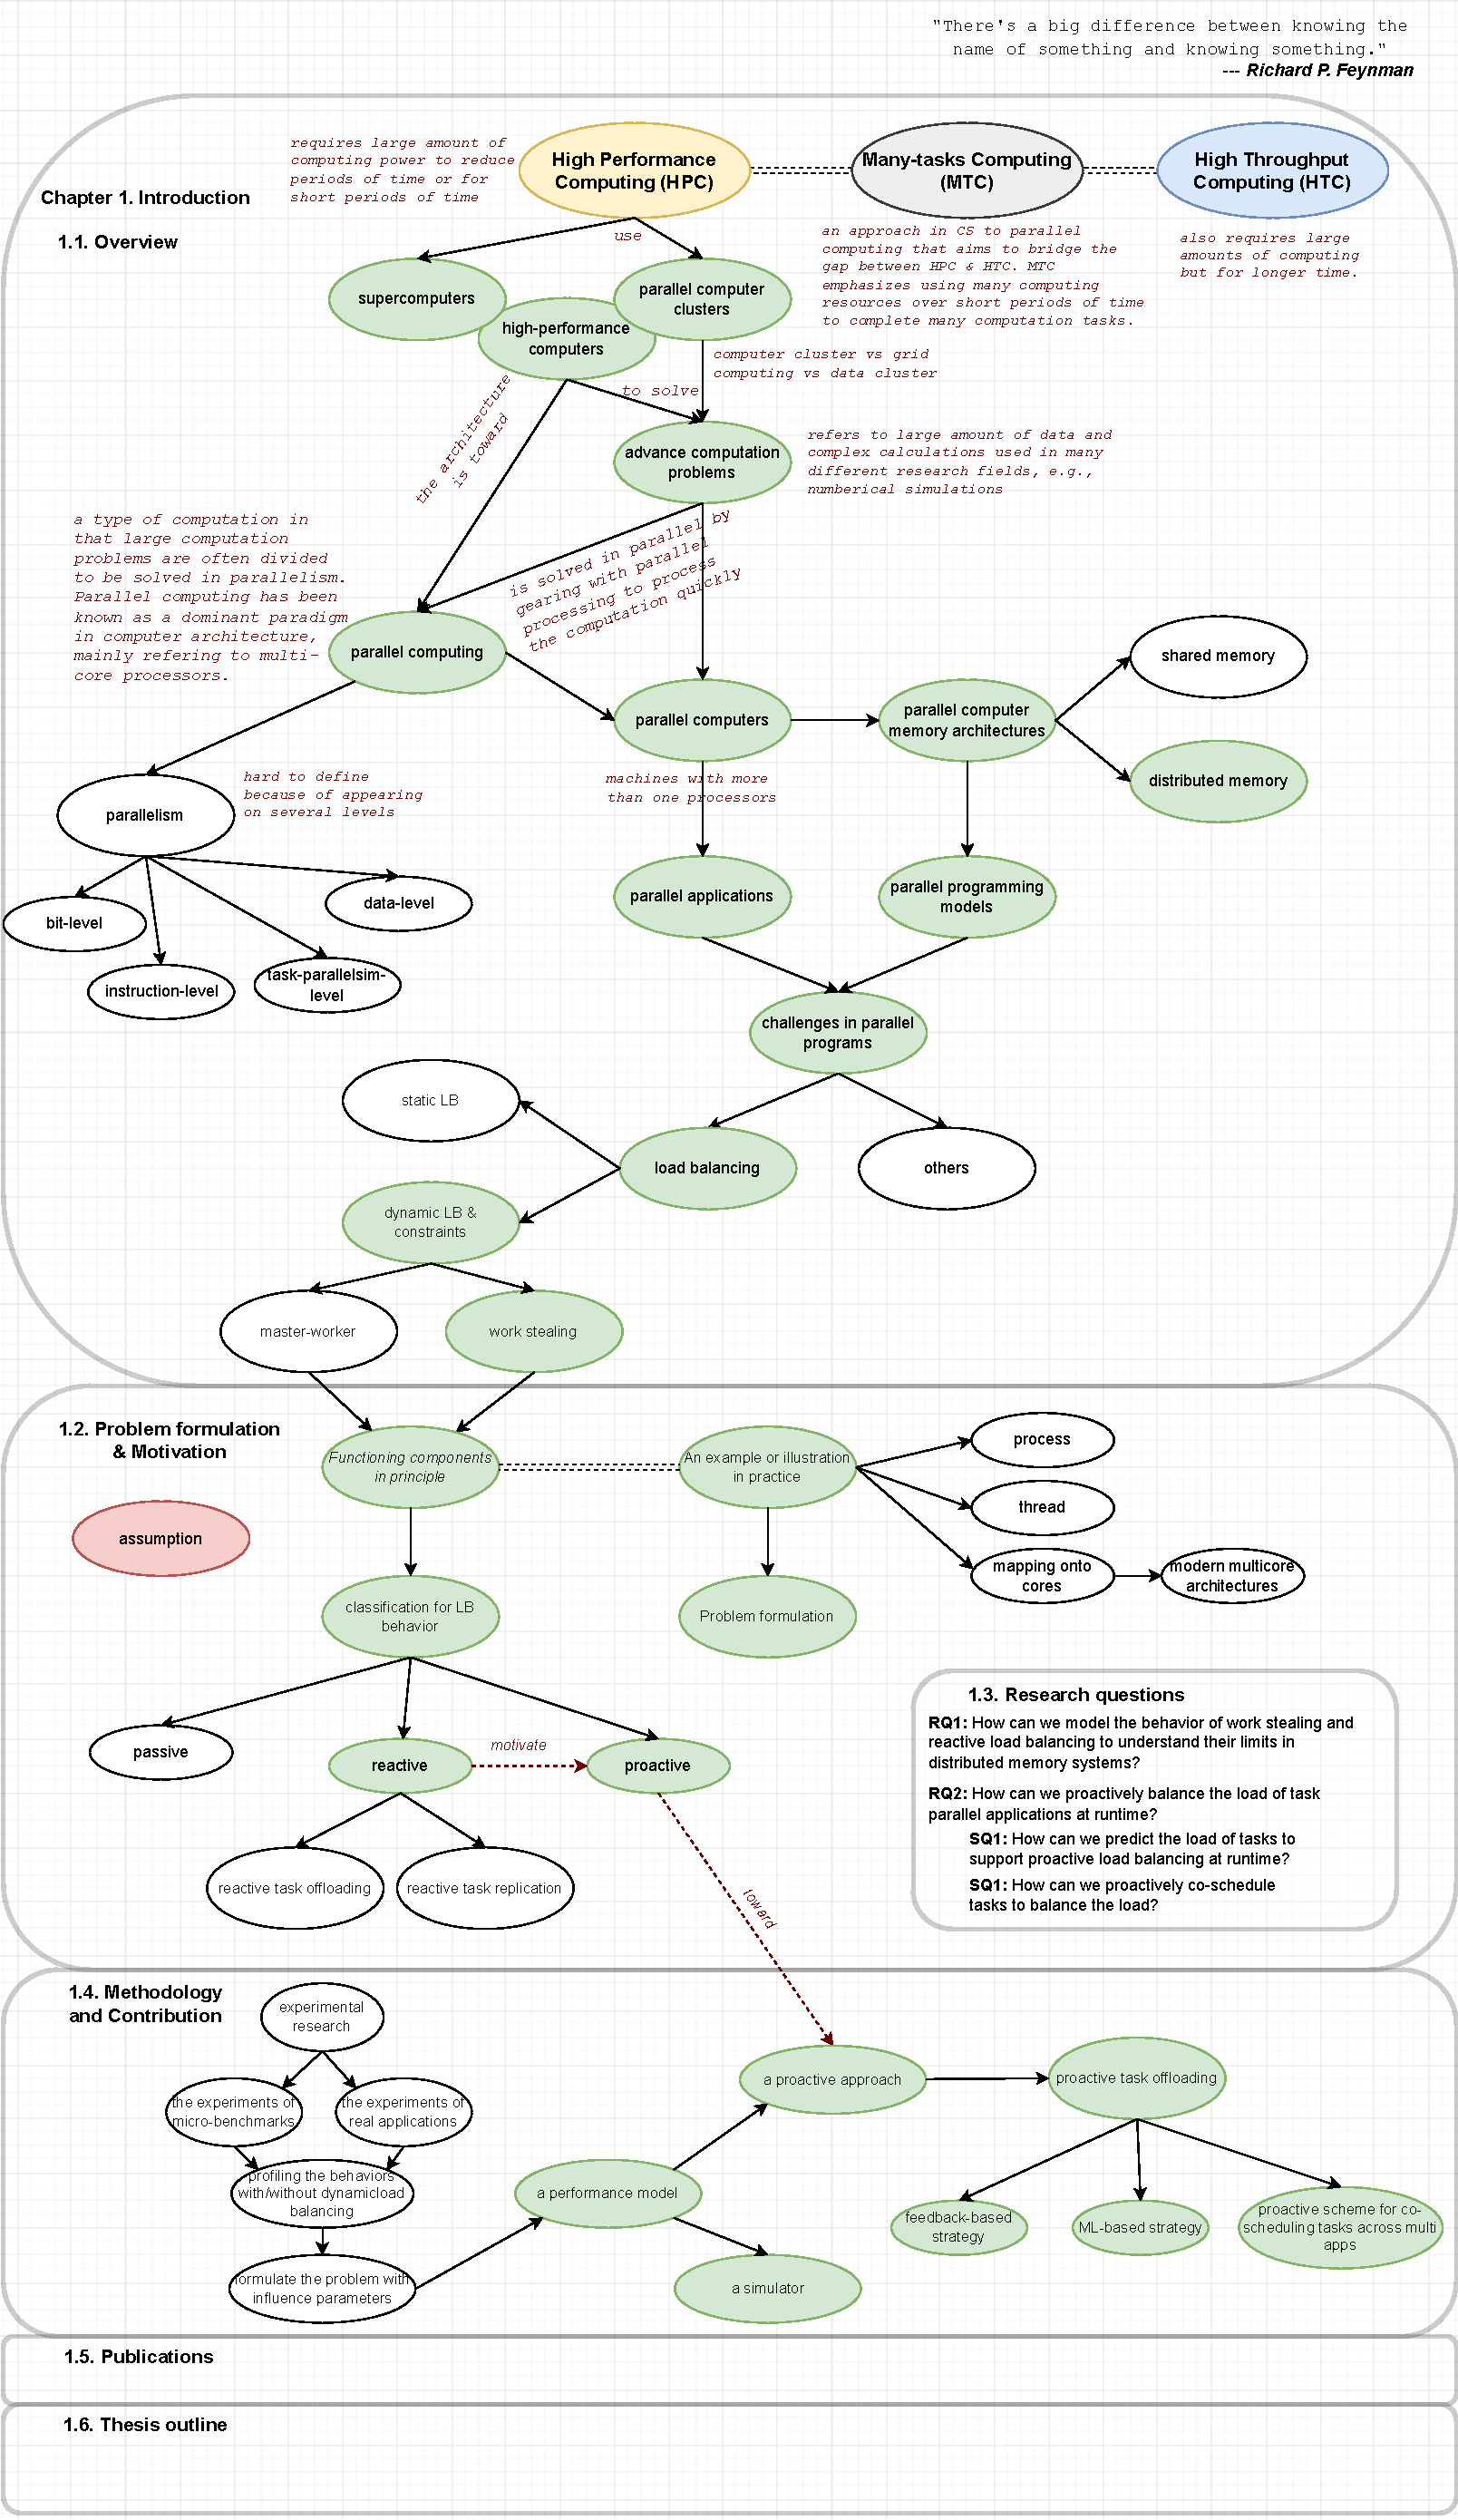
\includegraphics[scale=0.5]{./pictures/thesis_structure/taskflow_chapter1.pdf}
	\caption{Terms and key points in Chapter 1 represented as a taskflow.}
	\label{fig:thesistaskflow_chapter1}
\end{figure}


\begin{figure}[t]
  \centering
  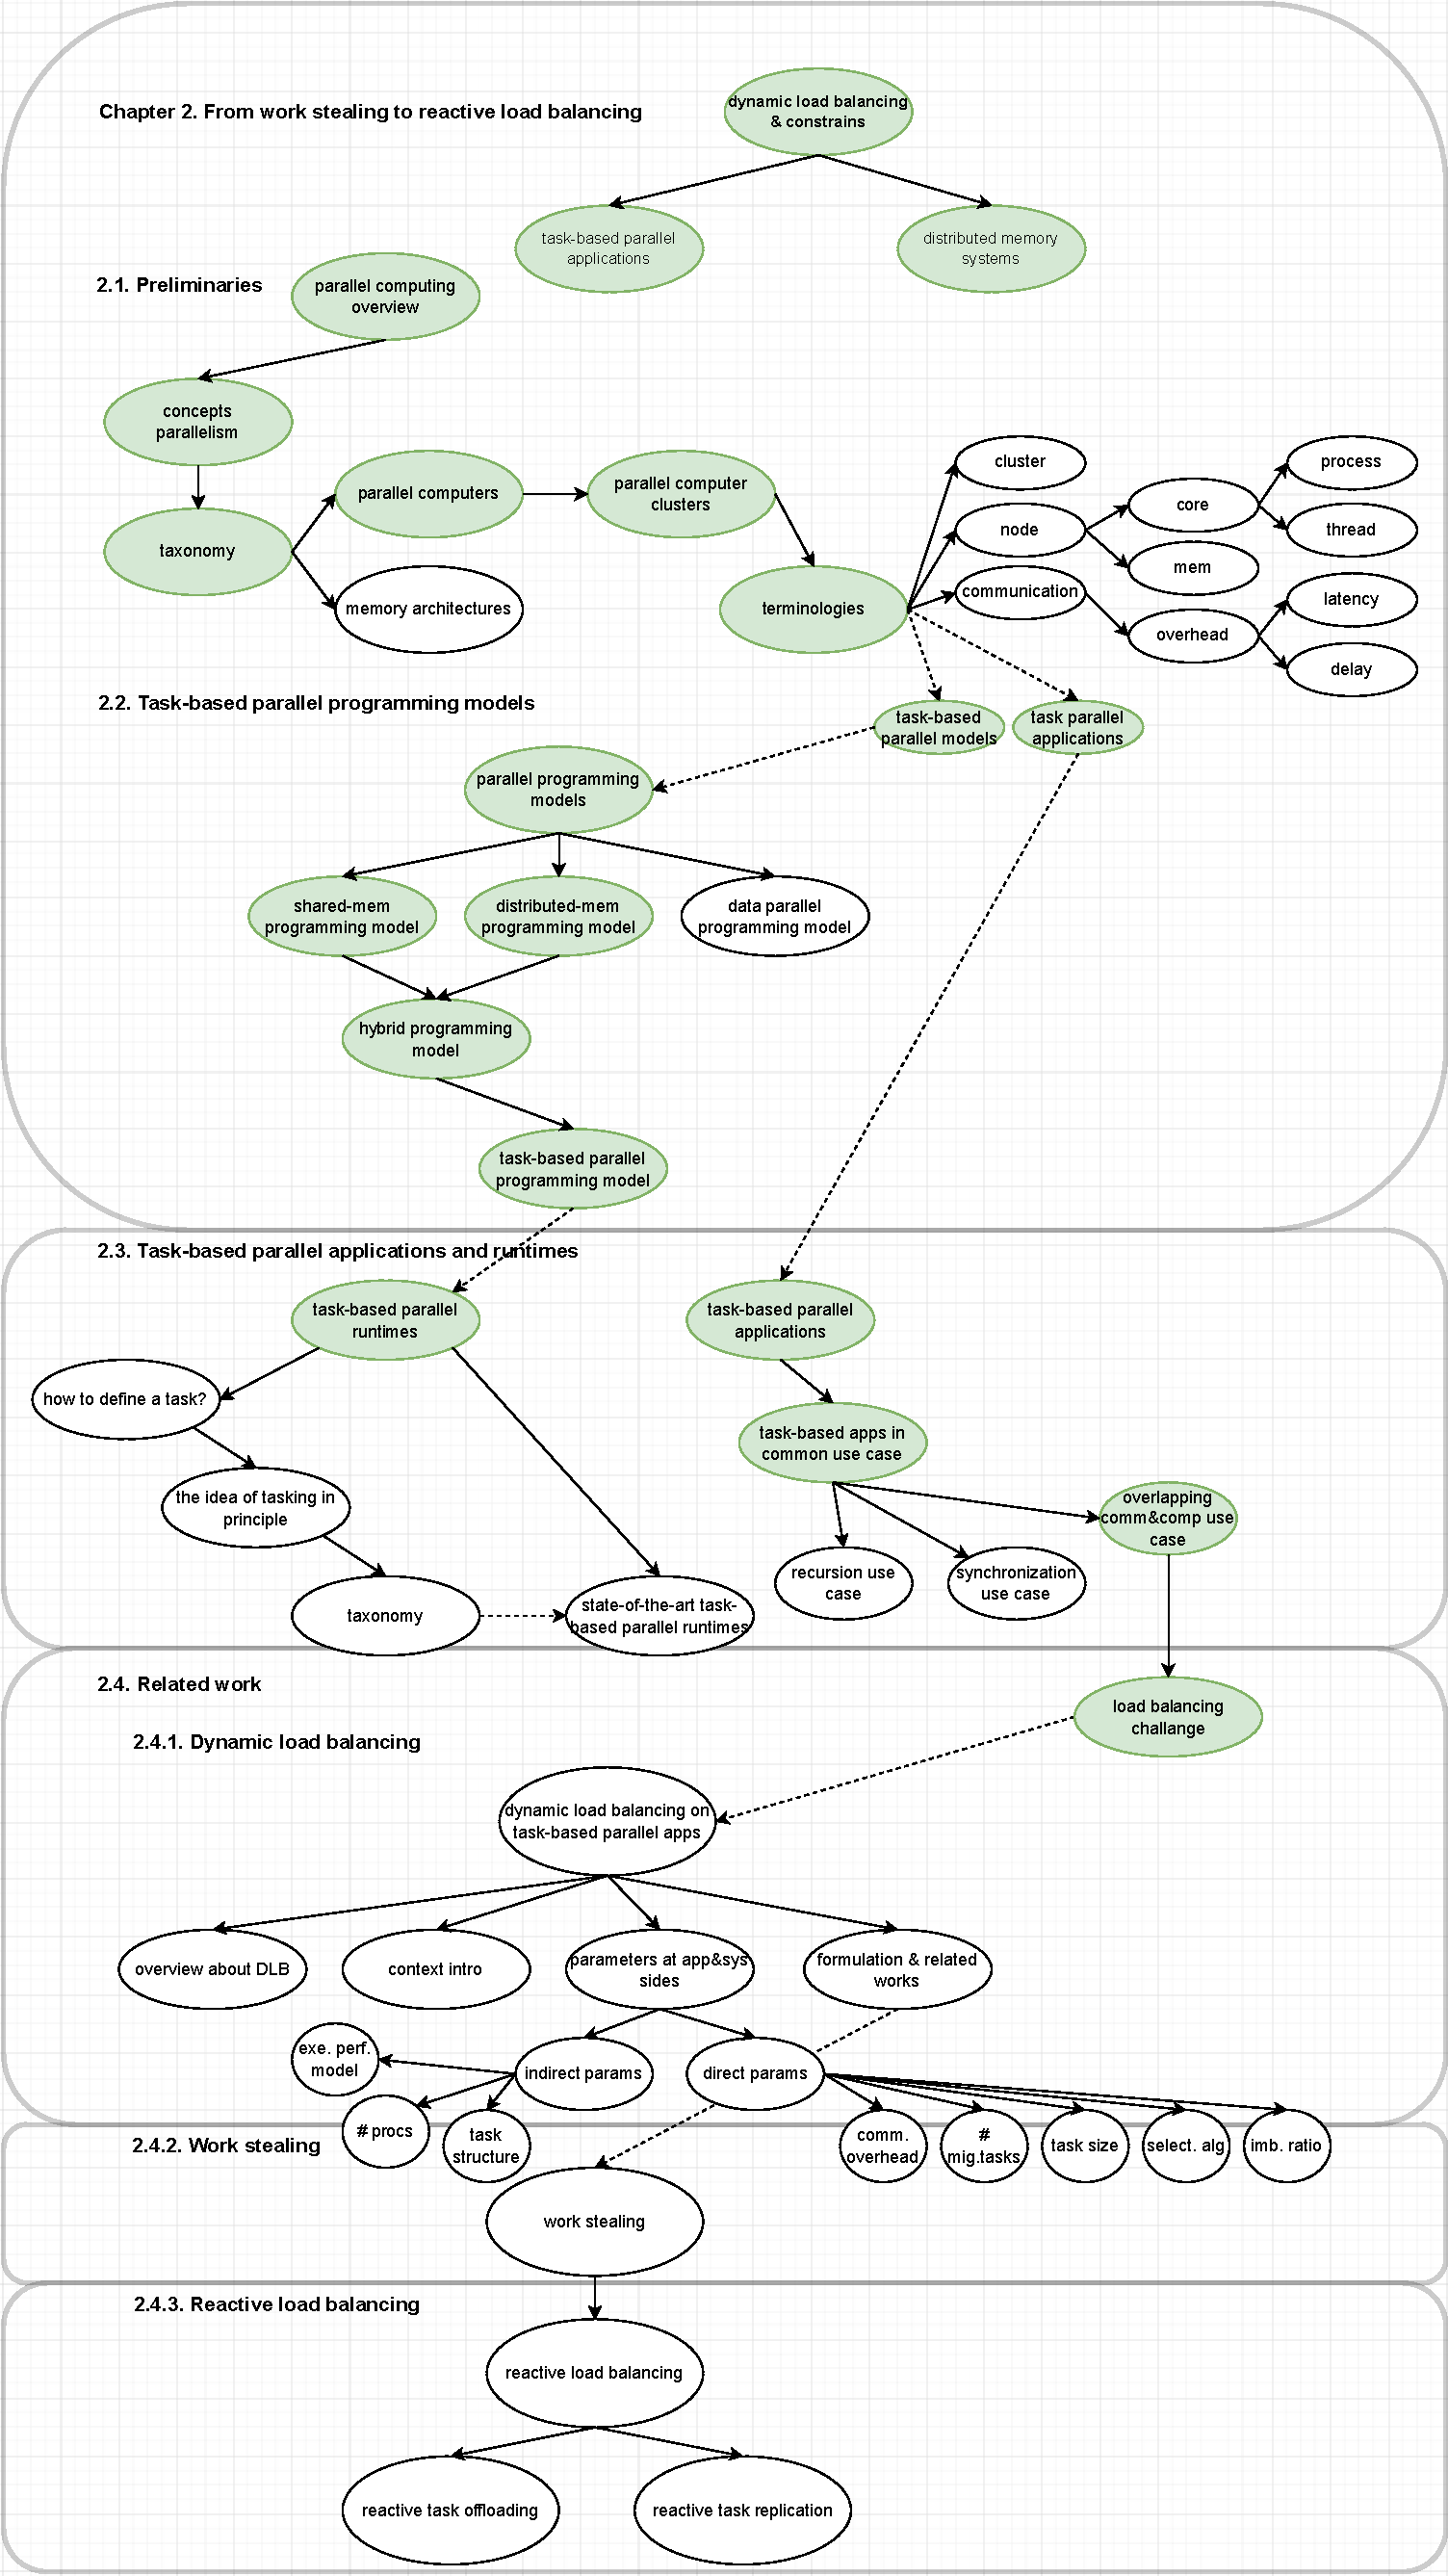
\includegraphics[scale=0.5]{./pictures/thesis_structure/taskflow_chapter2.pdf}
	\caption{Terms and key points in Chapter 2 represented as a taskflow.}
	\label{fig:thesistaskflow_chapter2}
\end{figure}


\begin{figure}[t]
  \centering
  \includegraphics[scale=0.5]{./pictures/thesis_structure/taskflow_chapter3.pdf}
	\caption{Terms and key points in Chapter 3 represented as a taskflow.}
	\label{fig:thesistaskflow_chapter3}
\end{figure}


\begin{figure}[t]
  \centering
  \includegraphics[scale=0.65]{./pictures/thesis_structure/taskflow_chapter4.pdf}
	\caption{Terms and key points in Chapter 4 represented as a taskflow.}
	\label{fig:thesistaskflow_chapter4}
\end{figure}


\begin{figure}[t]
  \centering
  \includegraphics[scale=0.45]{./pictures/thesis_structure/taskflow_chapter567.pdf}
	\caption{Terms and key points in Chapter 5, 6, 7 represented as a taskflow.}
	\label{fig:thesistaskflow_chapter567}
\end{figure}


%\section{Chapter 2 -- Related Work as a taskflow}
%\label{App_C_sec:relatedwork_taskflow}

%\section{Chapter 3 -- Performance Model as a taskflow}
%\label{App_C_sec:perfmodel_taskflow}

%\section{Chapter 4 -- Proactive Load Balancing as a taskflow}
%\label{App_C_sec:proactlb_taskflow}

%\section{Chapter 5-6-7 -- Proof of Concepts, Experiments, Conclusion and Future Work as a taskflow}
%\label{App_C_sec:chap567_taskflow}
